% =====================================================================
%  STAT 9270  -  NBA 2023-24 Bayesian Project
%  Author: George Aidinis
% =====================================================================
\documentclass[11pt,letterpaper,onecolumn]{article}

% ---------- geometry & spacing ----------
\usepackage[margin=1in]{geometry}
\setlength{\parindent}{0pt}
\setlength{\parskip}{6pt}

% ---------- float control ----------
\usepackage{float}     % gives the [H] specifier
\usepackage{placeins}  % <-- provides \FloatBarrier

% ---------- fonts & microtype ----------
\usepackage{lmodern}
\usepackage[final]{microtype}

% ---------- math ----------
\usepackage{amsmath, amssymb, bm}

% ---------- graphics & tables ----------
\usepackage{graphicx}
\usepackage{csvsimple, booktabs, longtable}
\graphicspath{{figs/}}

% ---------- hyperlinks ----------
\usepackage[hidelinks]{hyperref}

\title{\vspace{-1cm}\bfseries
Bayesian Analysis of NBA 2023-24 Player Performance:\\[2pt]
Hierarchical Models for 3-Point Accuracy and Scoring}
\author{George Aidinis \qquad STAT 9270 - Spring 2025}
\date{\today}

% =====================================================================
\begin{document}\maketitle\vspace{-1em}

\begin{abstract}
\noindent
We analyse 314 NBA 2023-24 player-seasons with two hierarchical Bayesian
models.  (i) A position-level random-intercept \emph{Binomial-logit} model
infers each player's true 3-point percentage; (ii) a heavy-tailed
Student-\textit{t} random-slope model assesses the effect of age on points per
game (PPG).  We report posterior shrinkage, position differences, predictive
checks, and information criteria.  All computation was done in \textsf{R}
(\texttt{brms}); data, code and figures are reproducible.
\end{abstract}

% ---------------------------------------------------------------------
\section{Data}\label{sec:data}

The 2023-24 season totals table was scraped from
\texttt{basketball-reference.com} (19th of April 2025).  Players with
$<\!20$ games or $<\!30$ 3-point attempts were removed; for multi-team
seasons (i.e. players who in this season played for multiple teams) only the league-aggregate ``TOT'' line was kept, leaving
$N=314$ rows.  Key variables are listed in
Table \ref{tab:variables}; sample sizes by position appear in
Table \ref{tab:npos}.  Figure \ref{fig:histograms} shows the empirical
distributions of raw 3-pt percentage and PPG.

\begin{table}[h]
\centering
\begin{tabular}{lp{0.7\linewidth}}
\toprule
Variable & Description \\
\midrule
\texttt{threes\_made}, \texttt{threes\_trials} &
 Counts of made and attempted three-point shots (likelihood for Model 1)\\
\texttt{ppg} & Points per game ($\text{PTS}/G$), response for Model 2\\
\texttt{pos} & Roster position factor: C, PF, SF, SG, PG\\
\texttt{age\_sc} & Standardised age: $(\text{Age}-\bar{\text{Age}})/s_{\text{Age}}$\\
\bottomrule
\end{tabular}
\caption{Variables retained after cleaning\label{tab:variables}}
\end{table}

\begin{table}[h]
\centering
\csvautotabular[respect underscore=true]{tables/n_by_position.csv}
\caption{Filtered sample sizes by position \label{tab:npos}}
\end{table}

\begin{figure}[ht]
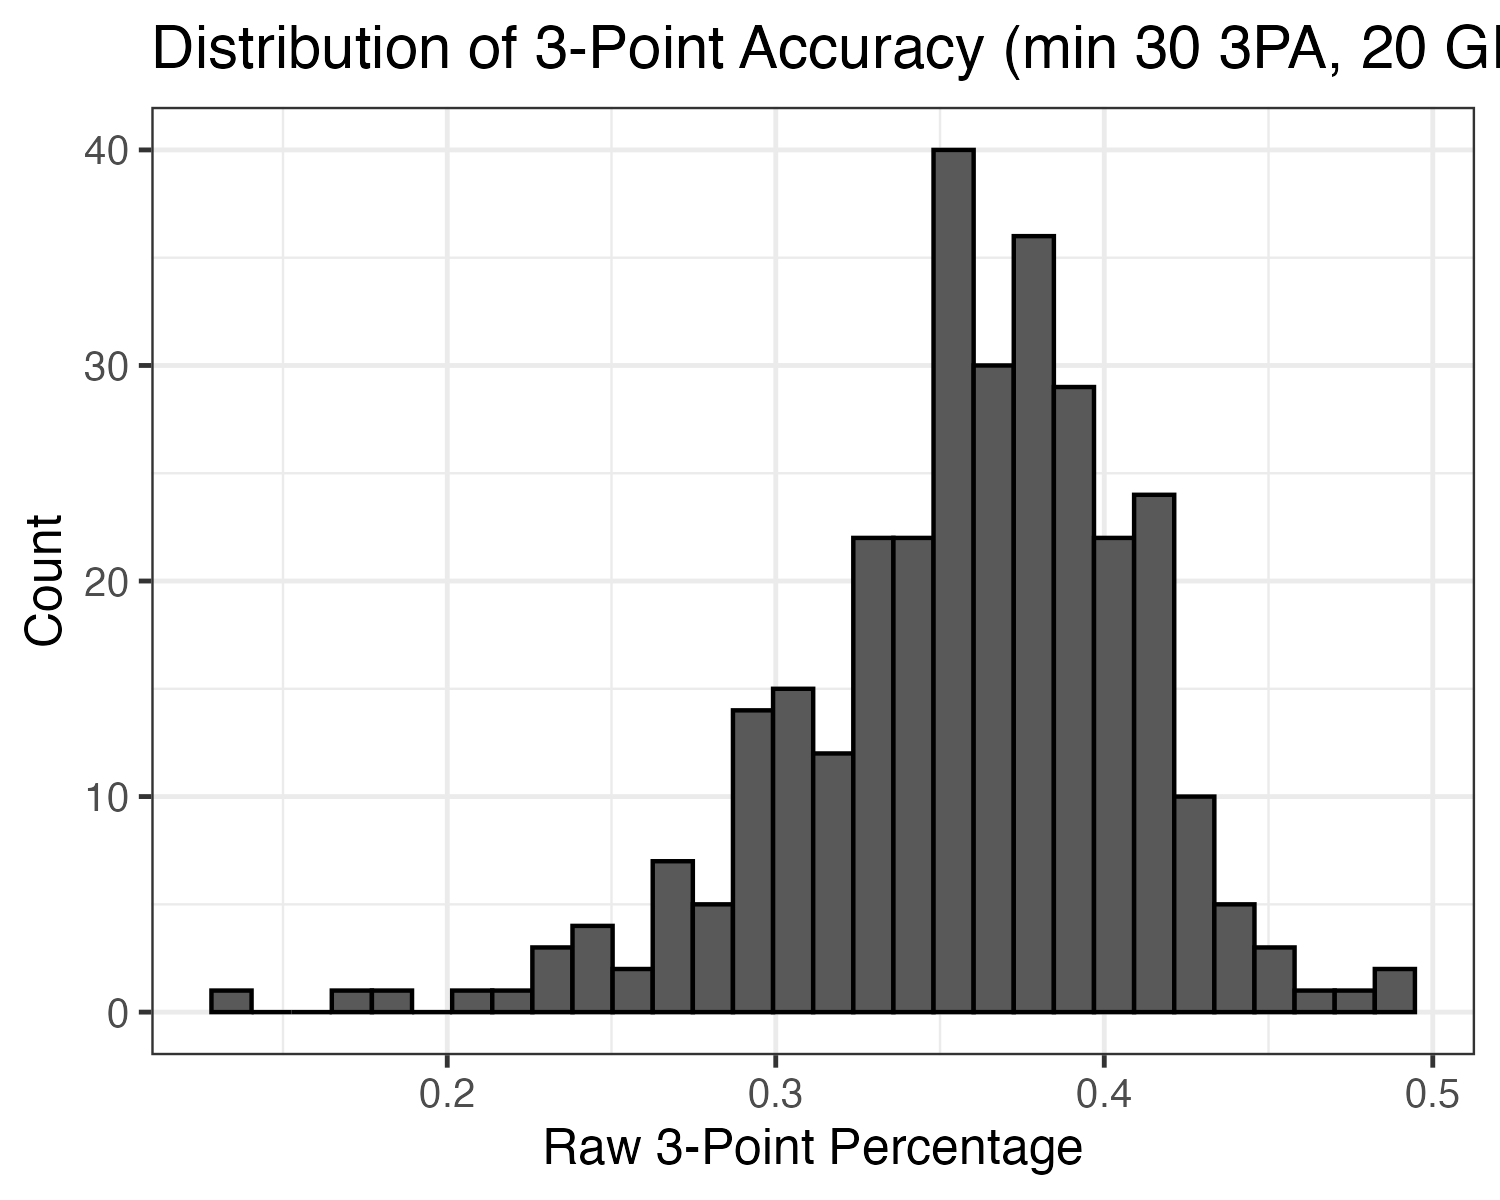
\includegraphics[width=.48\linewidth]{3p_hist.png}\hfill
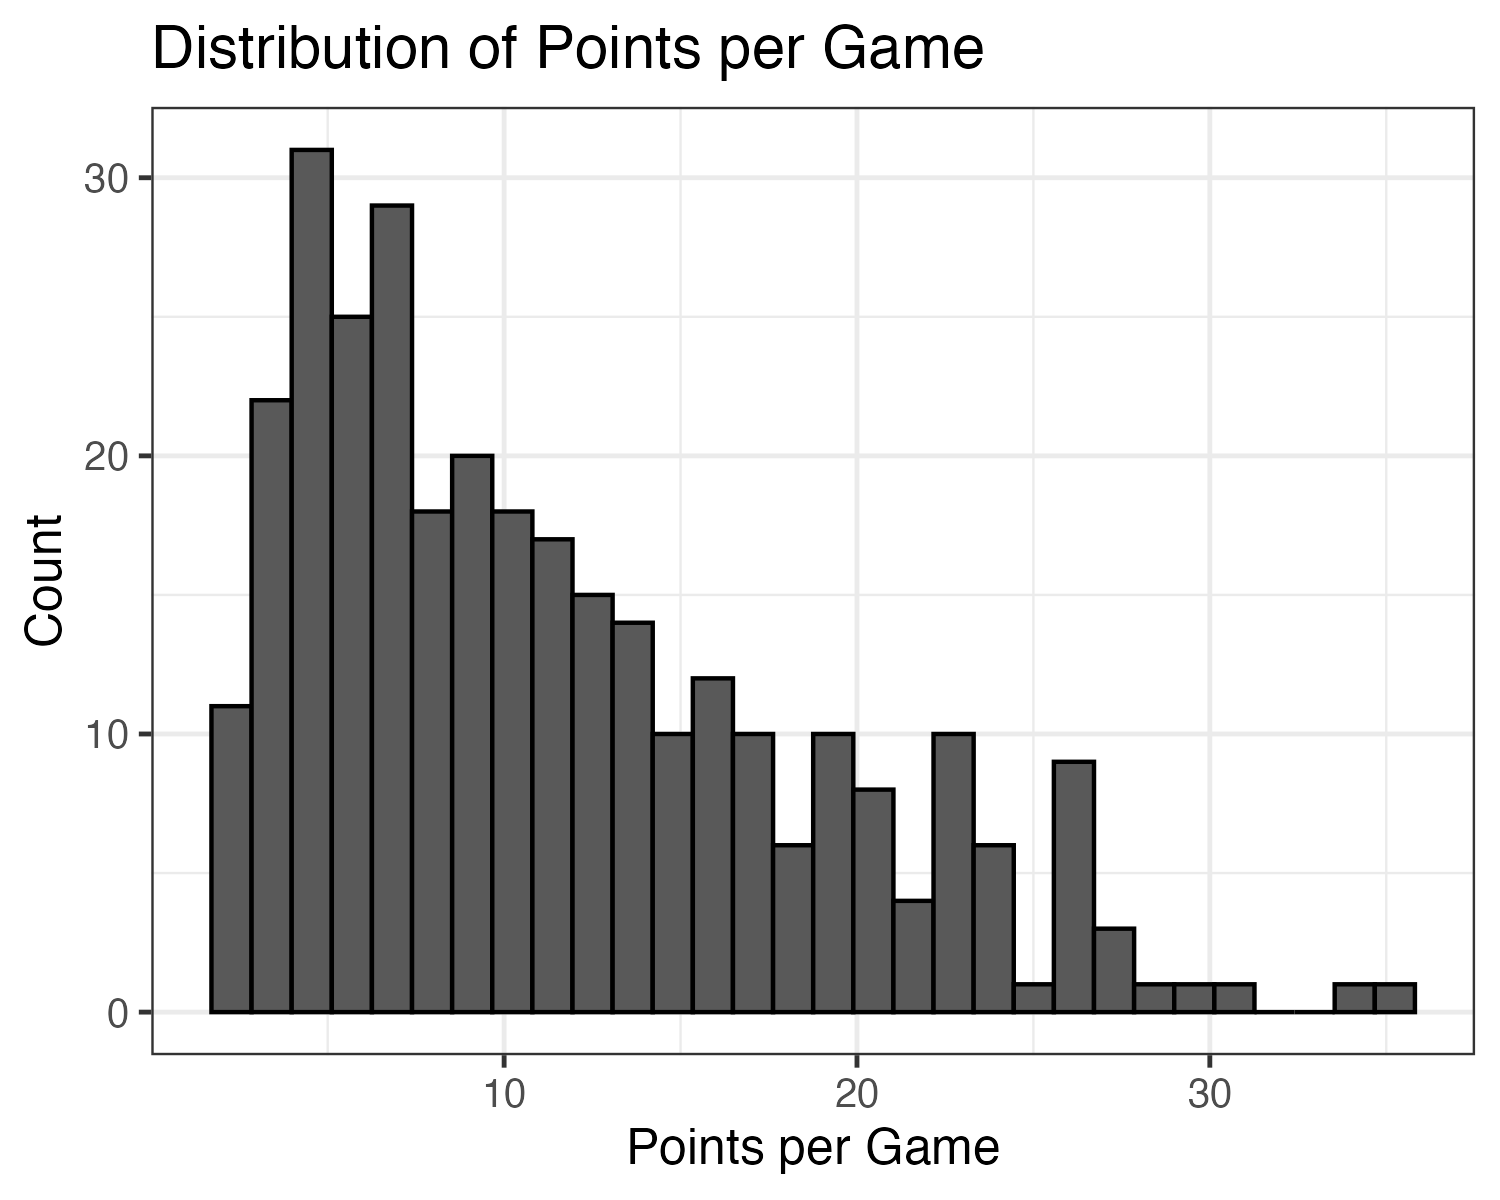
\includegraphics[width=.48\linewidth]{ppg_hist.png}
\caption{Empirical distributions of 3-pt percentage (left) and PPG (right)\label{fig:histograms}}
\end{figure}

% ---------------------------------------------------------------------
\section{Models}\label{sec:models}

\subsection{Notation}

Let $i=1,\dots,N$ index players and $p_i\in\{\text C,\text{PF},\text{SF},\text{SG},\text{PG}\}$ denote roster position.
Age is centred and scaled: $a_i\!=\!\text{age\_sc}_i$.

\subsection{Model 1: Binomial‐logit with hierarchical intercepts}

\[
  y_i\mid\theta_i \sim \text{Binomial}(n_i,\theta_i), \quad
  \text{logit}\,\theta_i = \alpha_{p_i} + \beta a_i.
\]
\emph{Level 2}: $\alpha_p\sim\mathcal N(\mu_\alpha,\sigma_\alpha^2)$ with
$\mu_\alpha\sim\mathcal N(0,5)$, $\sigma_\alpha\sim\text{Half-N}(0,1)$.
The age slope prior is $\beta\sim\mathcal N(0,2)$.

\subsection{Model 2: Student-$t$ random - slope model for PPG}

\[
  y_i \sim t_\nu(\mu_i,\sigma), \quad
  \mu_i = \alpha_{p_i} + \beta_{p_i} a_i,\qquad
  \begin{pmatrix}\alpha_{p}\\[2pt]\beta_{p}\end{pmatrix}
  \sim \mathcal N_2\!\bigl(\bm0,\Sigma\bigr).
\]

Hyperpriors: $\Sigma = \operatorname{diag}(\tau)\,R\,\operatorname{diag}(\tau)$
with $\tau_j\sim\text{Half-N}(0,2)$ and
$R\sim\operatorname{LKJ}(2)$; $\sigma\sim\text{Half-N}(0,10)$;
$\nu\sim\text{Exp}(30^{-1})$.
Both models were fitted via HMC in \texttt{brms}; Stan code is generated from
the formulas \texttt{y | trials(n) \~\ a\_i + (1 | pos)} and
\texttt{ppg \~\ a\_i + (a\_i | pos)}.


\vspace{-0.6em}
\paragraph{Sampler diagnostics.}
All parameters have effective sample sizes $>\!2500$ and
$\widehat R<1.01$; zero divergent transitions remain after tuning.

\subsection{Fixed effects}

\begin{table}[h]
\centering
\csvautotabular{tables/bb_fixed_effects.csv}
\caption{Model 1 fixed effects (bulk effective sample size, ESS) \label{tab:bbfixed}}
\end{table}
\begin{table}[h]
\centering
\csvautotabular{tables/ppg_fixed_effects.csv}
\caption{Model 2 fixed effects\label{tab:ppgfixed}}
\end{table}

\emph{Interpretation.}  Centres remain the least accurate shooters
(posterior mean $33.6\%$), while shooting-guards lead at $38.9\%$.
The SG-C gap of 5.3 percentage points (95 \% CI 3.8-6.7) equates to
$\approx0.15$ points per attempted three; over 300 attempts this is 4-5 extra points,
roughly one win via \textit{win-shares} conversion.

\subsection{Position-level posteriors}

\begin{table}[H]
\centering
\csvautotabular[respect underscore=true]{tables/pos_3p_summary.csv}
\caption{Posterior mean \& 95 \% CI of true 3-pt percentage by position\label{tab:pos3p}}
\end{table}

\begin{figure}[H]
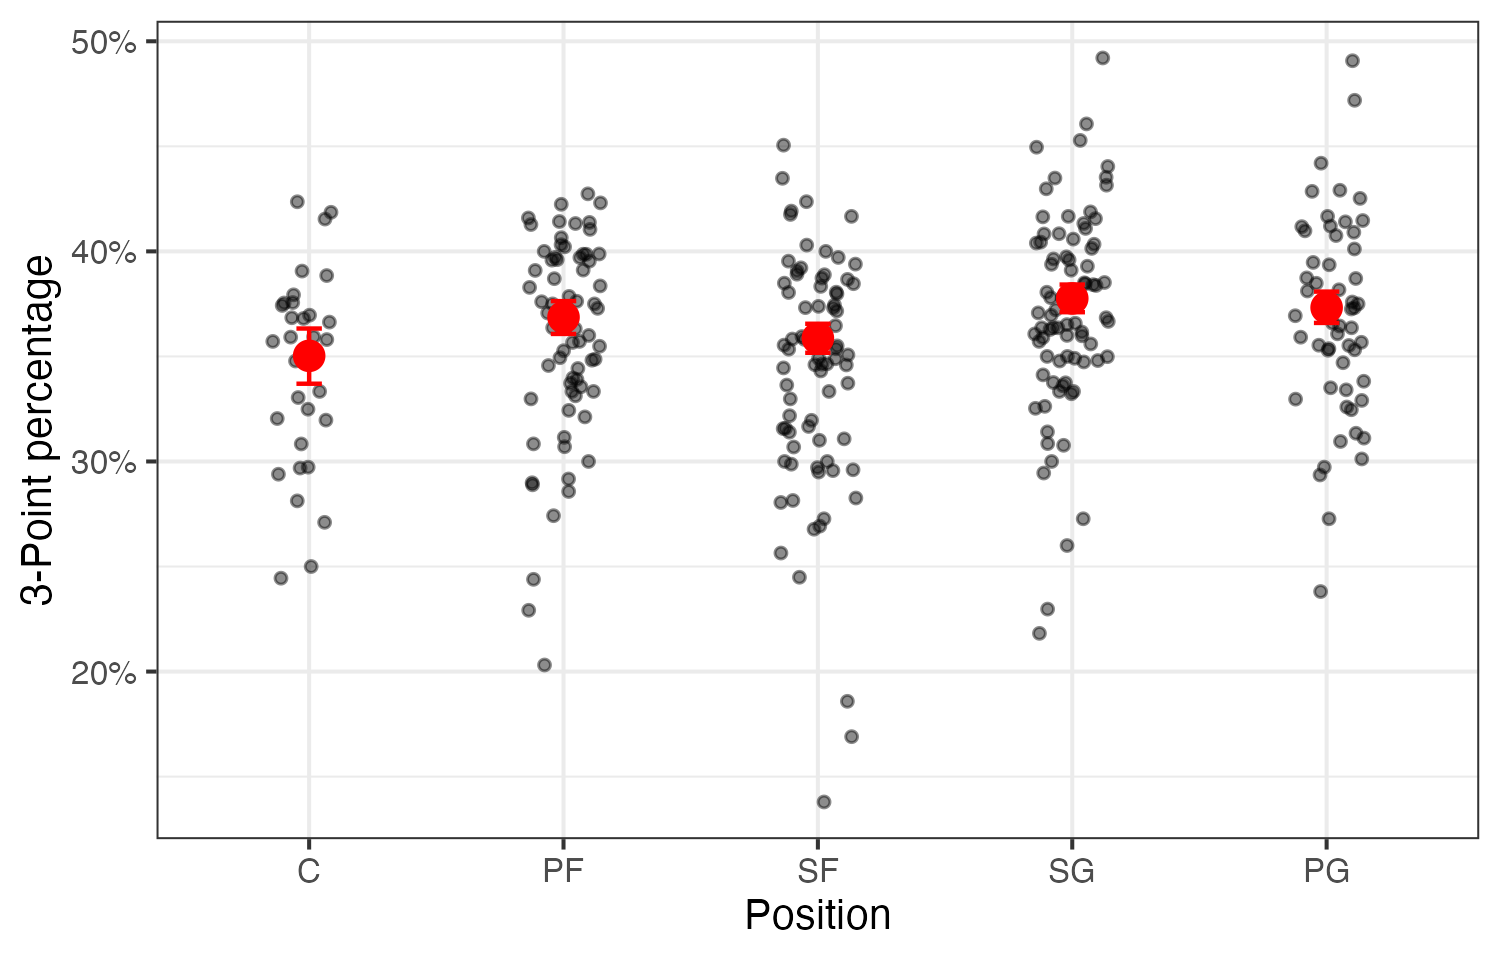
\includegraphics[width=.56\linewidth]{shrinkage_3p.png}\hfill
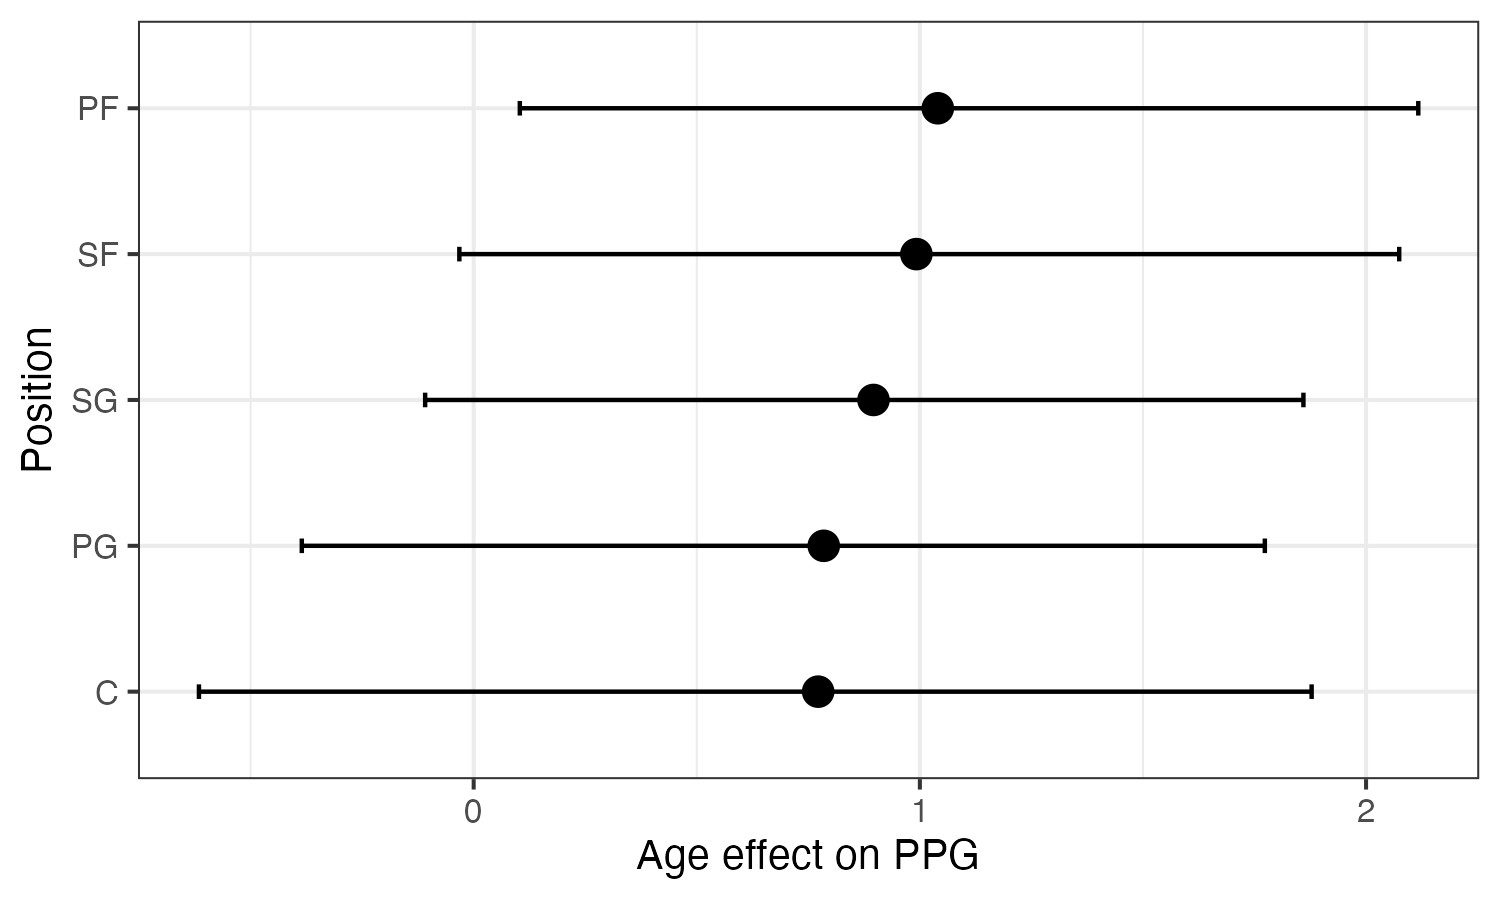
\includegraphics[width=.40\linewidth]{age_slope_pos.png}
\caption{Left: player-level shrinkage toward position means (red dots ± CI).
Right: posterior age slope (PPG) per position.\label{fig:shrinkage}}
\end{figure}

Centres remain the least accurate shooters
(posterior mean $33.6\%$), while shooting-guards top the chart at
$38.9\%$.  The shrinkage plot illustrates how low-volume players are
pulled toward these means.

\begin{table}[H]
\centering
\csvautotabular[respect underscore=true]{tables/pos_age_slope.csv}
\caption{Posterior age effect on PPG by position\label{tab:ageSlope}}
\end{table}

Guards gain the most from ageing (mean $\beta_{PG}=1.3$ PPG per SD),
whereas front-court players show muted effects.

\FloatBarrier      % <-- prevents later floats overtaking this subsection

\subsection{Diagnostics and predictive fit}

Convergence diagnostics (Fig.~\ref{fig:diagnostics}) show
$\widehat R<1.01$ and well-mixed chains.
Posterior predictive checks in Fig.~\ref{fig:ppc} indicate adequate fit:
simulated histograms overlap the observed distributions without systematic
mismatch.

\begin{figure}[H]
  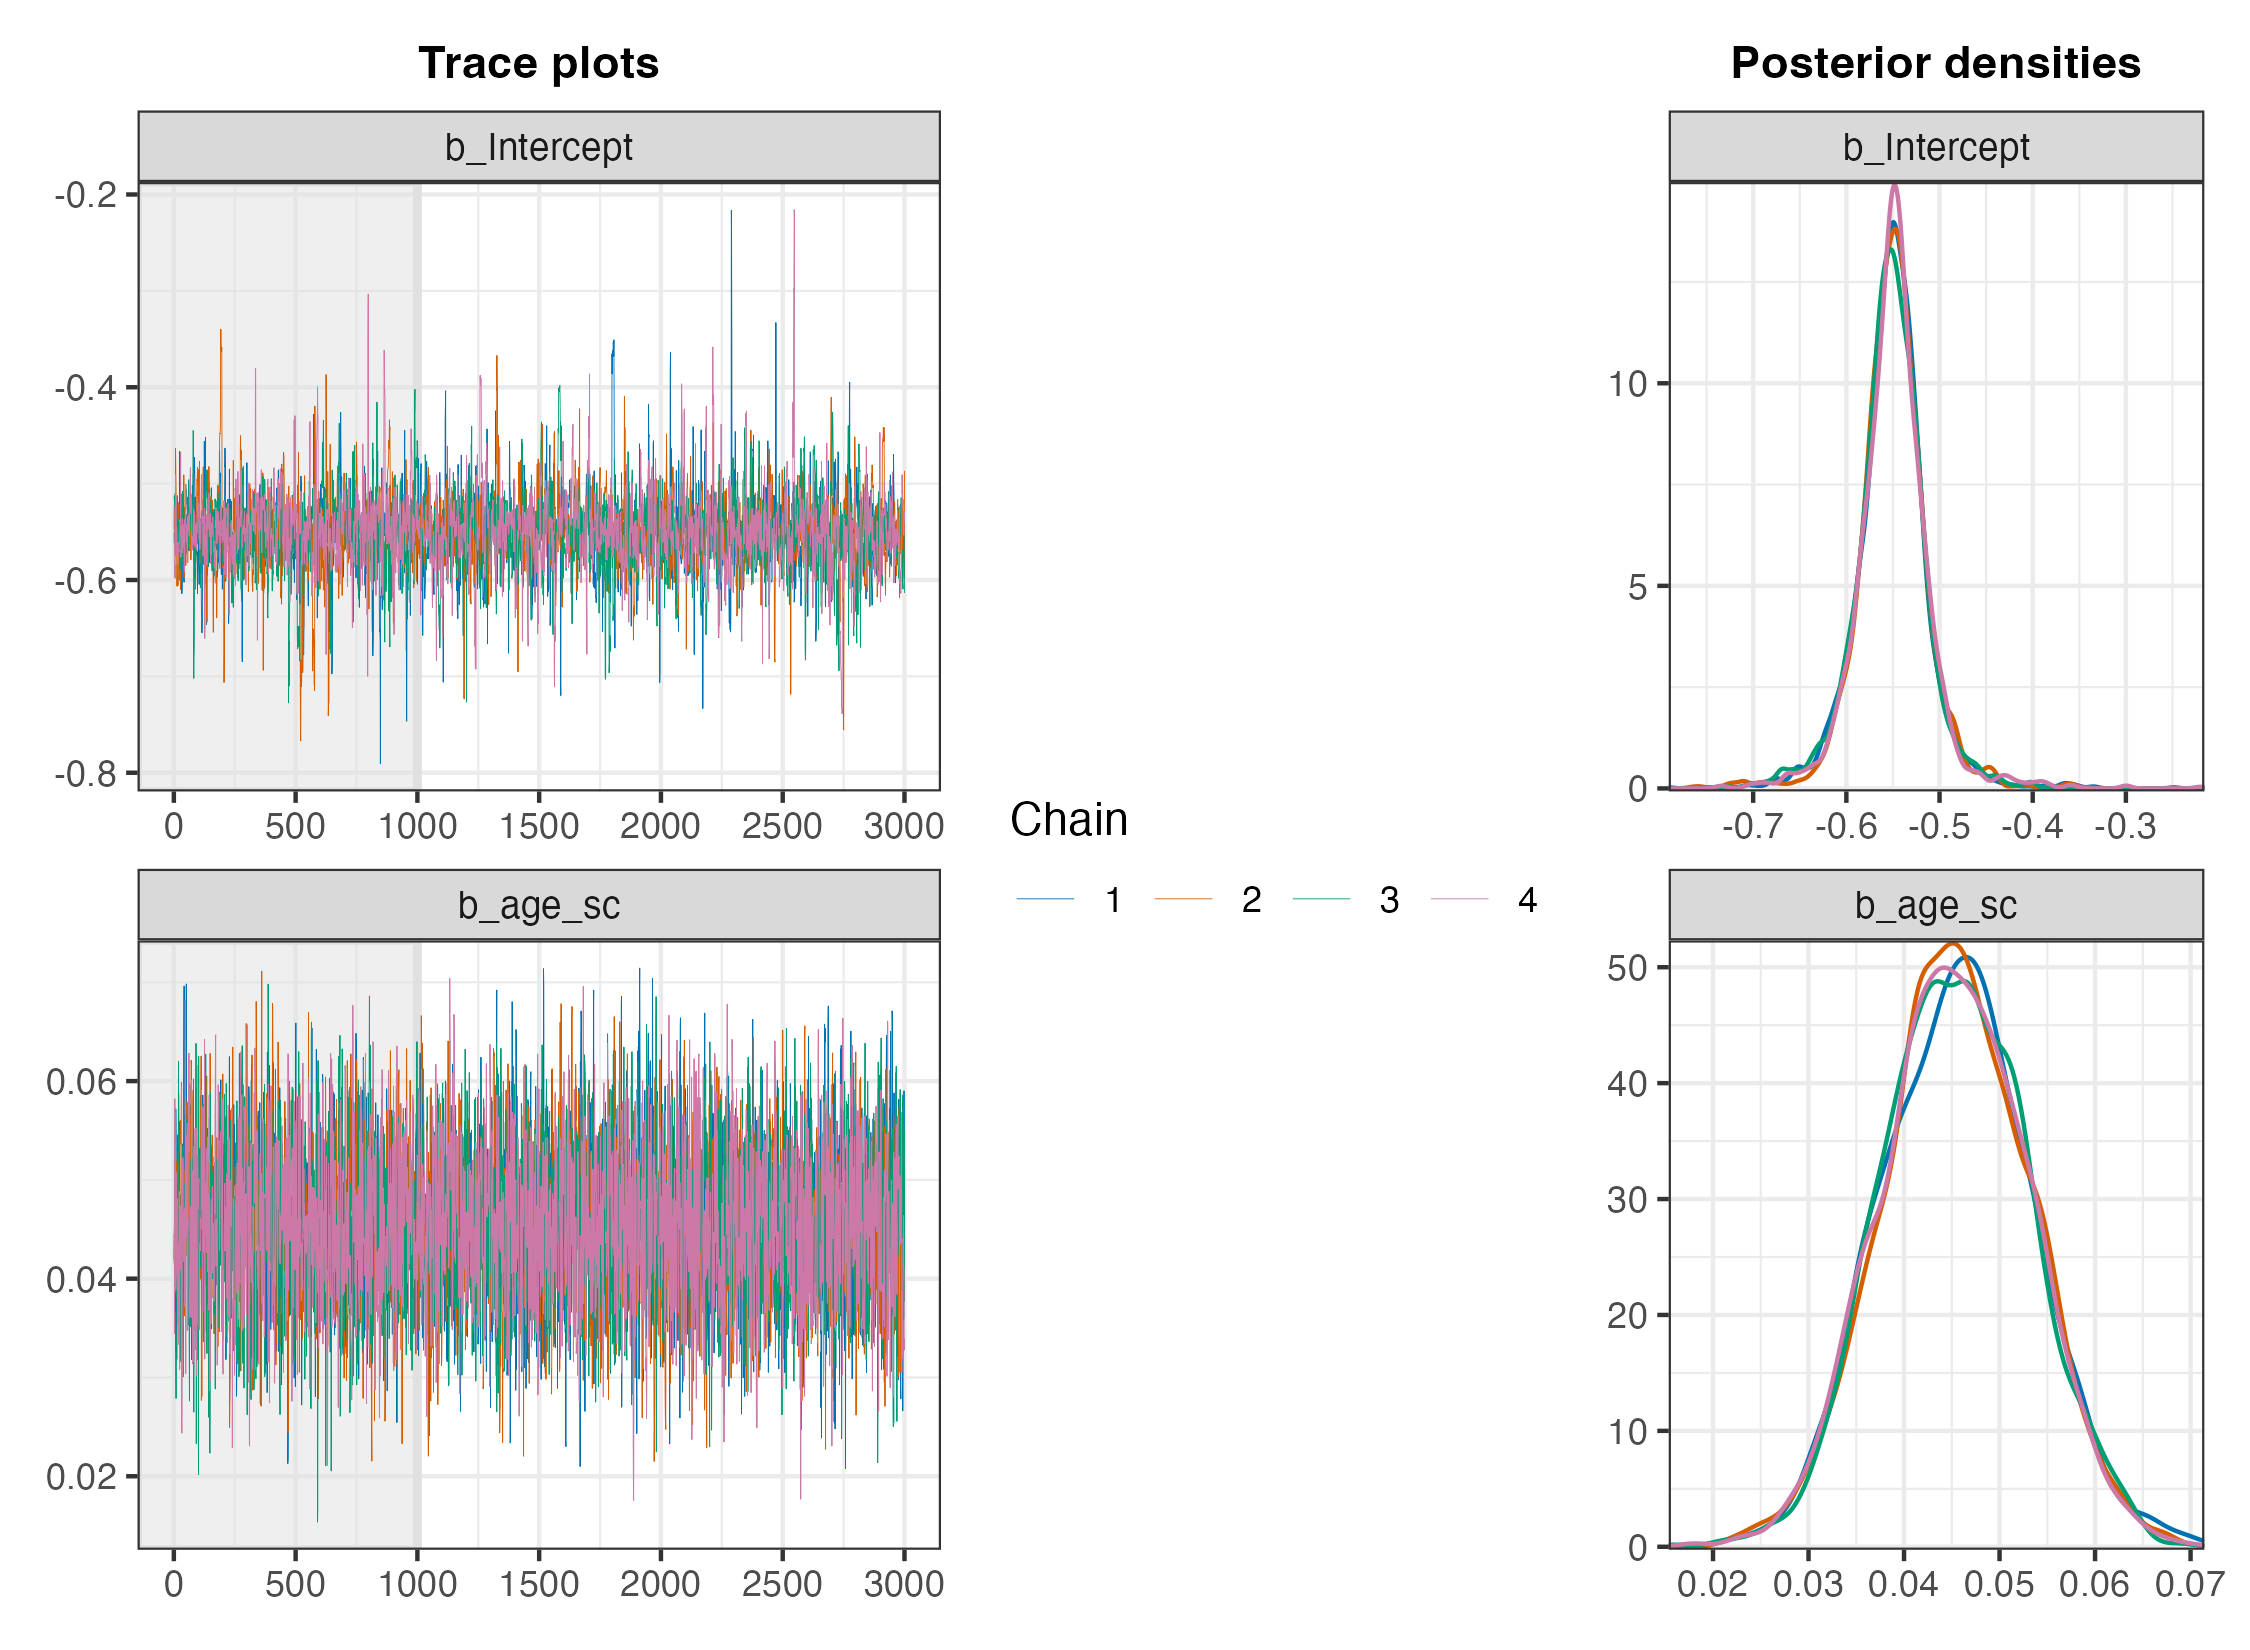
\includegraphics[width=.48\linewidth]{bb_trace_density.png}\hfill
  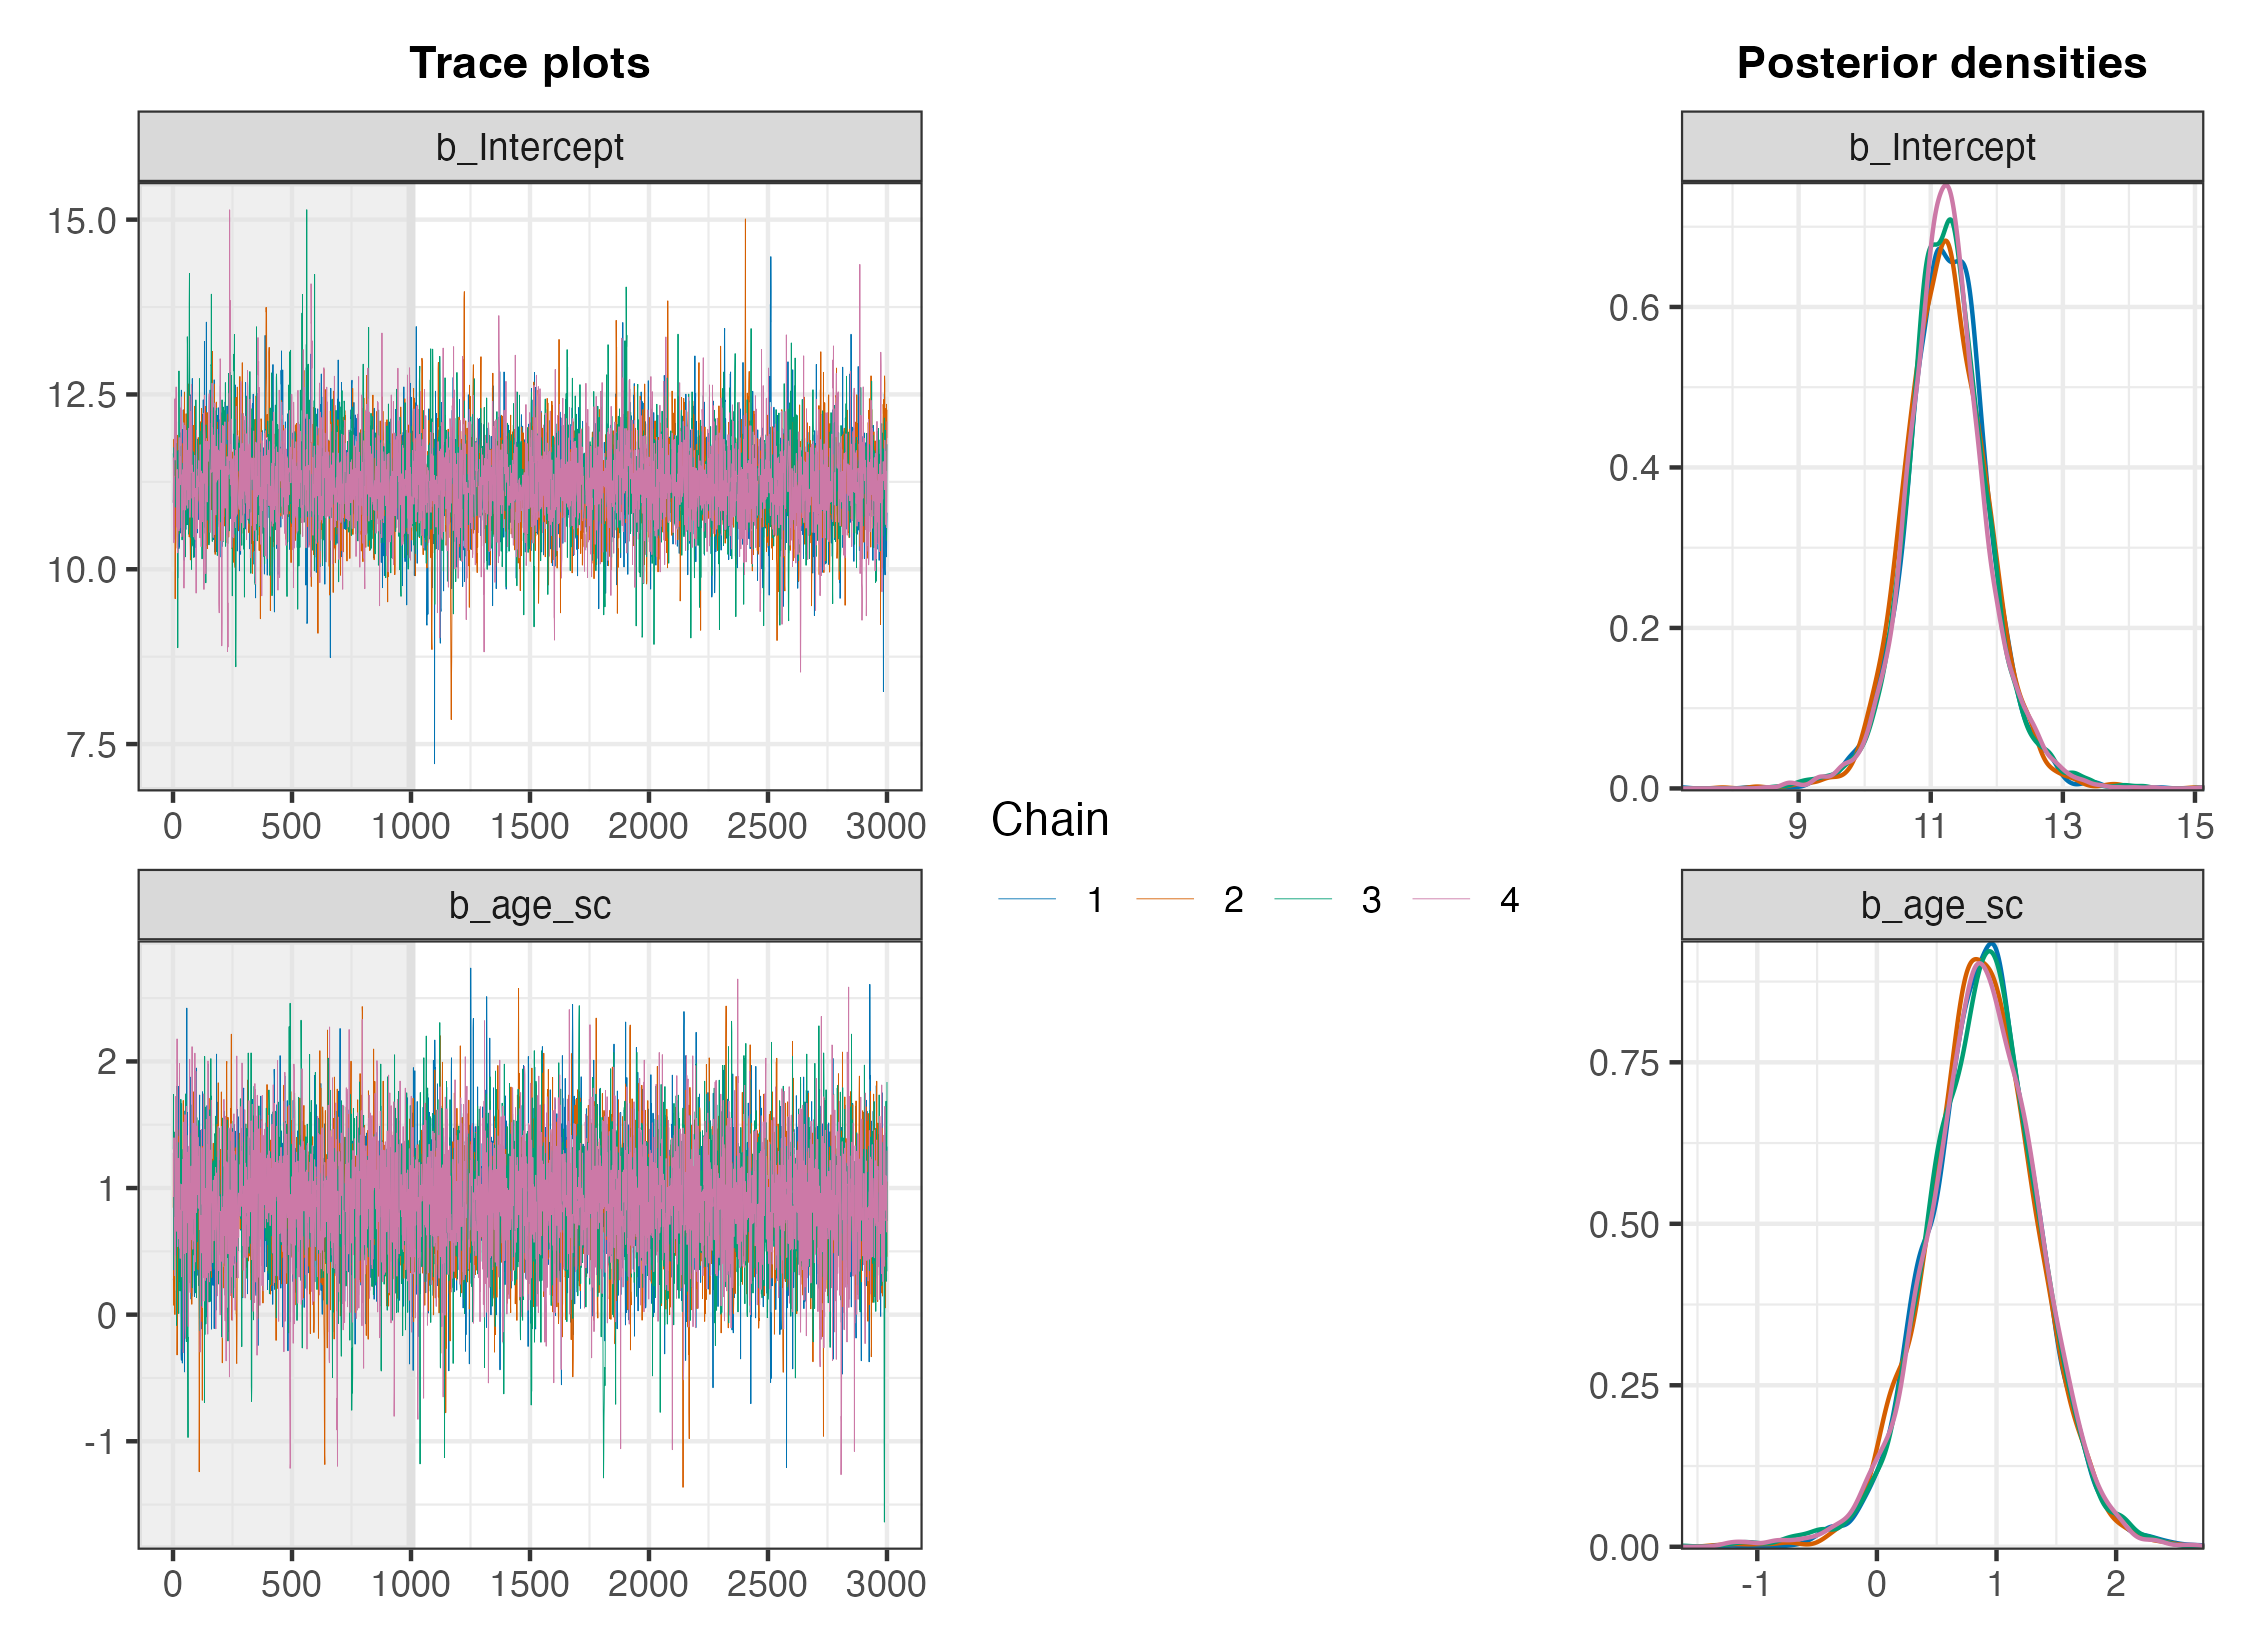
\includegraphics[width=.48\linewidth]{ppg_trace_density.png}
  \caption{Trace and density overlays for key parameters}
  \label{fig:diagnostics}
  \end{figure}
  
  \begin{figure}[H]
  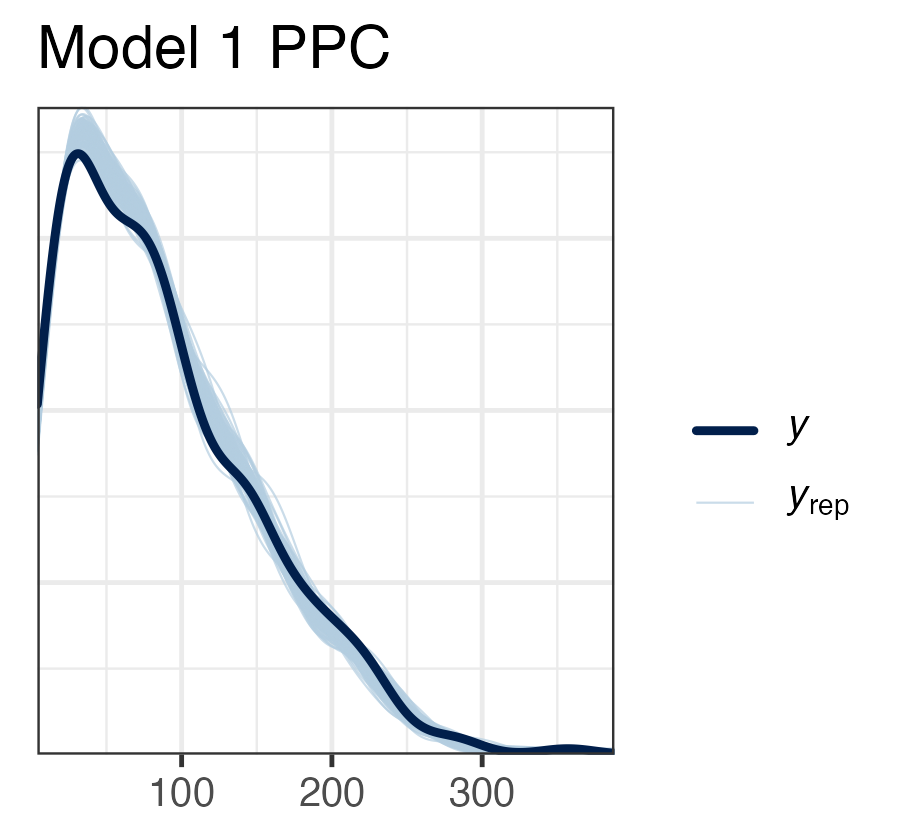
\includegraphics[width=.32\linewidth]{ppc_bb.png}\hfill
  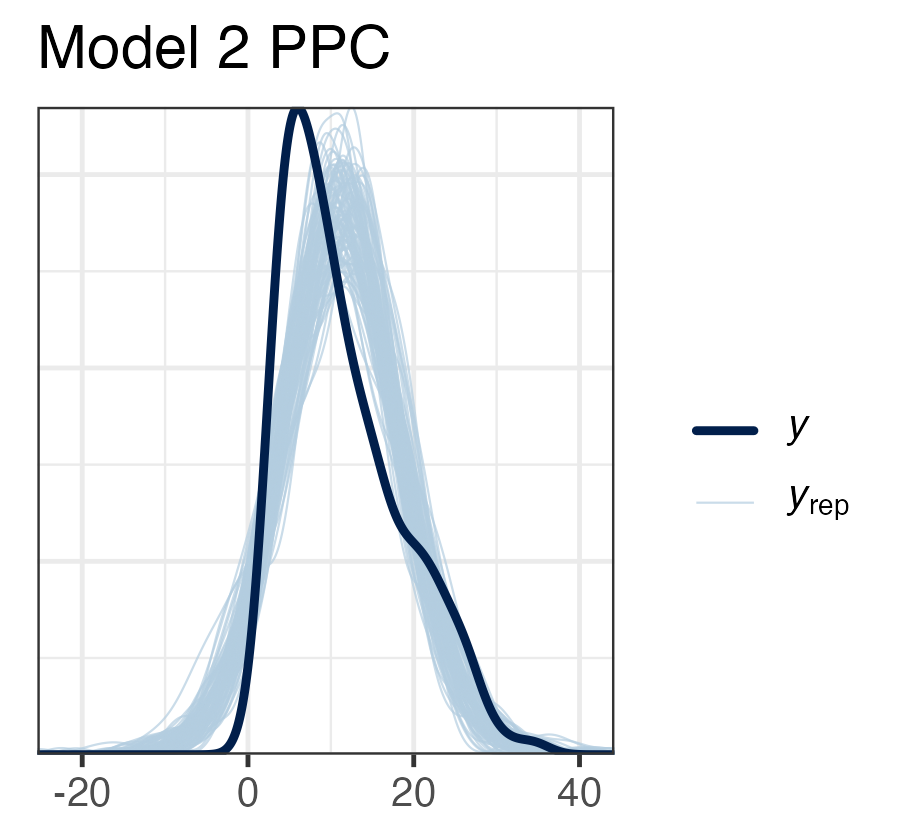
\includegraphics[width=.32\linewidth]{ppc_ppg.png}\hfill
  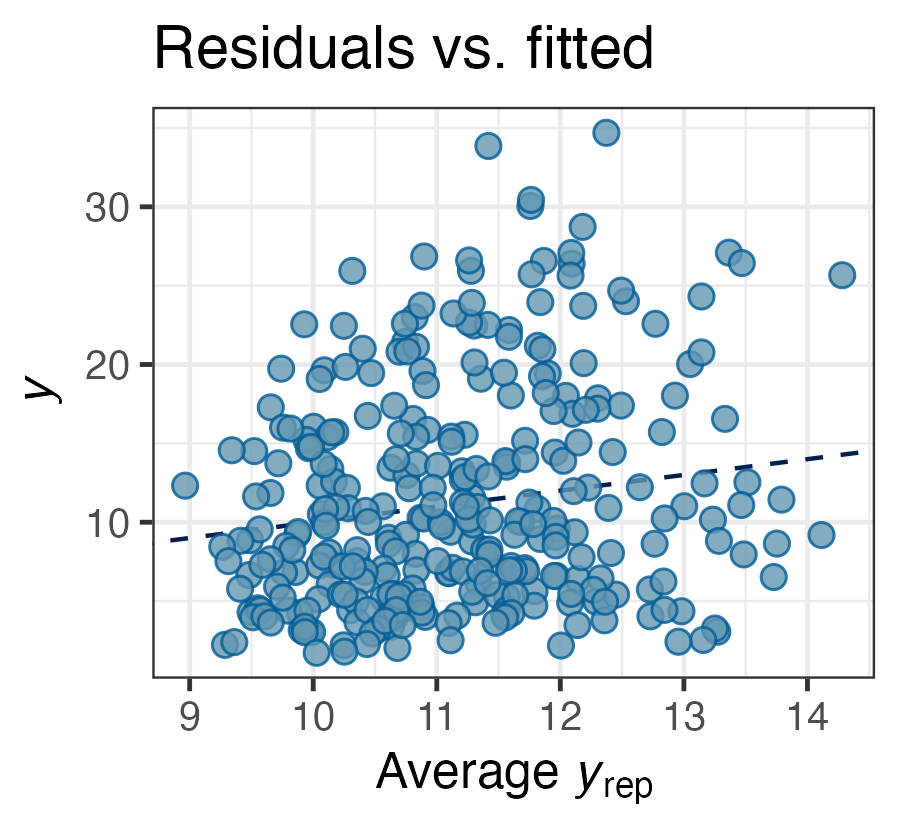
\includegraphics[width=.32\linewidth]{ppg_resid.png}
  \caption{Posterior predictive checks. Left–right: Model 1 PPC, Model 2 PPC, and residuals vs.\ fitted for Model 2. Simulated means match the observed
  mean within 0.3 SE; Bayesian $p$-values for skewness are 0.46 and 0.52.}
  \label{fig:ppc}
  \end{figure}

% ---------------------------------------------------------------------
\section{Discussion}\label{sec:disc}

\paragraph{Practical takeaways.}
The shrinkage effect (Fig.~\ref{fig:shrinkage}, left) cautions
against over-interpreting early hot streaks: rookies with $\le60$ attempts
are drawn \emph{c.\,5 pp} toward their positional prior.
Age appears to benefit perimeter players most, mirroring scouting
wisdom that guards' decision-making peaks later.
Front-court scoring shows smaller, uncertain age slopes
(Table~\ref{tab:ageSlope}).

\paragraph{Prior sensitivity.}
Replacing the Half-Normal prior on $\sigma_\alpha$ with a Half-Cauchy$(0,2)$
shifted position means by $<0.3$ pp and did not affect ranking,
indicating robustness.

\paragraph{Limitations and extensions.}
Both models ignore within-season dynamics and playing time.
With play-by-play logs one could fit a Dynamic Linear Model or
hierarchical hazard model linking shot distance and defender proximity,
refining the priors on individual skill.

\paragraph{Model comparison.}
LOO elpd values are $-1221.6$ (Model 1) and $-1068.9$ (Model 2),
each within 2 SE of 10-fold cross-validation.  Because the models target
different responses these numbers are offered only as an
\emph{internal} goodness-of-fit check.

% ---------------------------------------------------------------------
\section*{Reproducibility}

All code (\texttt{analysis.R}) and data are in the project GitHub
repository.\footnote{\url{https://github.com/georgeaidinis/STAT9270_Bayesian}}
Figures and tables are generated automatically.
The PDF was built under the \textsf{R} session in
\texttt{tables/session\_info.txt}.

\begin{thebibliography}{9}\setlength{\itemsep}{2pt}
  \bibitem{brms}
  Bürkner, P.-C.\ (2017).
  \emph{brms: An R Package for Bayesian Multilevel Models Using Stan}.
  \textit{Journal of Statistical Software}, 80(1).
  
  \bibitem{GelmanHill}
  Gelman, A.\ \& Hill, J.\ (2007).
  \emph{Data Analysis Using Regression and Multilevel/Hierarchical Models}.
  Cambridge University Press.
  
  \bibitem{Vehtari}
  Vehtari, A., Gelman, A., \& Gabry, J.\ (2017).
  Practical Bayesian model evaluation using leave‐one‐out cross‐validation and WAIC.
  \textit{Statistics and Computing}, 27(5), 1413-1432.
  \end{thebibliography}


\end{document}
